\chapter{\texorpdfstring{$L_0-$}{Lg}Regularized Regression with Correlated Features}
\label{cha:L0}

\section{Introduction}
In chapter \ref{cha:introduction},  we discussed the feature selection properties of the lasso, elastic net, and best subset selection. The latter is equivalent to $L_0$ constrained regression when data matrix $\bm{X}$ is orthogonal. In fact, the lassso and elastic net can be thought of as approximation methods to best subset selection. We see this in section \ref{sec:nonconvex}; in the spectrum of $L_q$ constrained regression, $q=0$ corresponds to best subset selection, $0<q<1$ to nonconvex regularization, $q=1$ to the lasso, and $q=2$ to ridge regression, which does not perfom selection. As the value of $q$ moving away from 0 to larger values, the estimated regression coefficients become more biased toward 0, and the resulting model becomes less sparse. Under orthogonality of the design matrix, best subset selection ($L_0$) yields unbiased coefficient estimates. Therefore, $L_0$ constrained regression would be generally the preferred model. However, in reality the features are not orthogonal, and exhibit some degree of correlations. In this situation, the $L_0$ constrained regression is an NP-hard problem \citep{huo2007stepwise}. 

Several approaches have been proposed for fitting the $L_0$-regularized linear regression. \cite{blumensath2008iterative} introduced an iterative hard thresholding algorithm, which is a proximal gradient-based method. Based on hard thresholding, several variants of the method have also been developed, such as proximal iterative hard thresholding \citep{zhang2019new}, and proximal alternating iterative hard thresholding \citep{yang2017proximal}. These methods share the main idea of applying the proximal operator univariately to obtain coordinate-wise solutions. However, these methods ignore the correlation structure of the data matrix $\bm{X}$, and might not work well with correlated features. We look at a novel algorithm to $L_0$ constrained least squares  and modify it to incorporate the covariance matrix $\bm{X}^T\bm{X}$ into account. The original plan for this work was to later extend $L_0$ constrained least squares to integrate meta-features. However, the approach did not work as expected and we turned to the methods in Chapters 2 and 3 instead. We include it here for completion and because some of the ideas may prove useful in the future.

\section[Proximal distance algorithm for \texorpdfstring{$L_0-$}{Lg}regularized regression]{Proximal distance algorithm for \texorpdfstring{$L_0-$}{Lg}regularized regression}
Proposed by \cite{keys2019proximal}, the proximal distance algorithm is a general method for solving a constrained optimization problem. It converts a constrained minimization problem into an unconstrained one, with a penalty on the distance to the constrain set. The constrained minimization problem is 
\begin{equation} \label{prox_con}
\begin{aligned}
    & \min_{x\in \mathbb{R}^p} f(x), \\
    & \text{subject to} \hspace{0.6cm} x\in C, 
\end{aligned}
\end{equation}
where $C$ is a closed set. This general constrained optimization problem can be turned into a penalized version (unconstrained)
\begin{equation} \label{prox_uncon}
   \min_{x\in \mathbb{R}^p} f(x)+\frac{\rho}{2}\text{dist}(x,C)^2,
\end{equation}
where the squared distance is defined as $\text{dist}(x,C)^2=\inf_{y\in C}\|x-y\|_2^2$, i.e. the square of the Euclidean distance of $x$ to the closed set $C$. The distance penalty function is nonnegative and vanishes precisely on $C$. As the penalty parameter $\rho$ tends to $\infty$, the distance of $x$ to set $C$ is penalized so strongly that it is close to 0, i.e., $x$ is in the set, which means the minimizer found by the unconstrained version \eqref{prox_uncon} is equivalent to the constrained one \eqref{prox_con}. To minimize \eqref{prox_uncon}, we again use a majorization-minimization (MM) algorithm similar to that used in chapter \ref{cha:xtunecox} to estimate the model hyperparameters. The majorization step, which forms an upper bound of $f(x)$ around the current iterate $x_n$, replaces the distance penalty function $\text{dist}(x,C)^2$ with the spherical quadratic $\|x-P_C(x_n)\|_2^2$, where $P_C(x_n)$ is the projection of the $n^{th}$ iterate $x_n$ onto C: the point in set C that attains the minimum distance to the point, $P_C(x_n)=\argmin_{x\in C}\|x_n-x\|_2$. Therefore, by the definition of projection, $\|x-P_C(x_n)\|_2^2\geq\text{dist}(x,C)^2$, and at current iterate $x_n$, the tangency condition, $\|x_n-P_C(x_n)\|_2^2=\text{dist}(x_n,C)^2$ of a majorization is satisfied. The minimization step is then the proximal map of the current projection
\begin{equation}
    x_{n+1}=\text{prox}_{\rho^{-1}f}(P_C(x_n))=\argmin_x f(x)+\frac{\rho}{2}\|x-P_C(x_n)\|_2^2.
\end{equation}
The MM principle guarantees that $x_{n+1}$ decreases the penalized loss.

For the $L_0$-regularized least squares problem, the constrained optimization form can be written as 
\begin{equation} \label{L0_con}
    \begin{aligned}
    \min_{\beta\in \mathbb{R}^p} \frac{1}{2}\|y-\bm{X}\beta\|_2^2, \\
    \text{subject to} \hspace{0.6cm} \beta \in S_k^p,
    \end{aligned}
\end{equation}
where $S_k^p$ is the set of vectors with at most $k$ nonzero entries out of $p$. The unconstrained form of \eqref{L0_con}, i.e., the penalized distance objective function is
\begin{equation} \label{L0_uncon}
    \min_{\beta\in \mathbb{R}^p} \frac{1}{2}\|y-\bm{X}\beta\|_2^2+\frac{\rho}{2}\text{dist}(\beta, S_k^p)^2.
\end{equation}
To use the majorization-minimization algorithm to solve problem \eqref{L0_uncon}, first we perform distance majorization
\begin{equation}
    \min_{\beta\in \mathbb{R}^p} \frac{1}{2}\|y-\bm{X}\beta\|_2^2+\frac{\rho}{2}\|\beta-P_{S_k^p}(\beta_n)\|_2^2.
\end{equation}
The minimization step is the proximal operator of the projection onto set $S_k^p$,
\begin{equation}
    \beta_{n+1}=\text{prox}_{\rho^{-1}\text{OLS}}(P_{S_k^p}(\beta_n))=(\bm{X}^T\bm{X}+\rho\bm{I})^{-1}(\bm{X}^Ty+\rho P_{S_k^p}(\beta_n)).
\end{equation}
We discussed earlier that the distance penaly parameter $\rho$ should be increased systematically until a constrained minimum is reached. In practice, starting $\rho_0=1$, and increasing its value through a sequence $\rho_n=\min(\alpha^n\rho_0, \rho_{\max})$ with  $\alpha$ slightly larger than 1 works well. The overall algorithm can be summarized as follow:
\begin{enumerate}
    \item Initialize $\beta_0=1$, $\rho_0=1$, $\text{dist}_0=\infty$, $\text{loss}_0=\infty$,
    \item For iteration counter $n$ from $1$ to max iteration:
    \begin{enumerate}
        \item Update $\beta_n=\text{prox}_{\rho^{-1}OLS}(P_{S_k^p}(\beta_{n-1}))$
        \item Current distance $\text{dist}_n=\|\beta_n-P_{S_k^p}(\beta_{n-1})\|_w^2$
        \item Current loss function vaue $\text{loss}_n=OLS(\beta_n)$
        \item If $|\text{dist}_n-\text{dixt}_{n-1}|<\text{tolerance}$ and $|\text{loss}_n-\text{loss}_{n-1}|<\text{tolerance}$:
        \begin{itemize}
            \item break
            \item return $P_{S_k^p}(\beta_n)$
        \end{itemize}
        else:
        \begin{itemize}
            \item $\text{dist}_{n-1}=\text{dist}_n$
            \item $\text{loss}_{n-1}=\text{loss}_n$
            \item increase $\rho$ by a small multiplier $\alpha$ every few iterations
        \end{itemize}
    \end{enumerate}
\end{enumerate}

\section{Incorporating the data covariance matrix}
The proximal distance algorithm uses the Euclidean distance as the distance metric. But this ignores the correlations between features. To incorporate the covariance matrix, we can use the weighted distance (Mahalanobis distance):
\[
d(x,y)=\sqrt{(x-y)^T\bm{W}^{-1}(x-y)},
\]
where, assuming the columns of $\bm{X}$ are mean-centered, $\bm{W}=\bm{X}^t\bm{X}$ is the data covariance matrix. With weighted distance majorization, the new update is 
\begin{equation}
    \beta_{n+1}=\text{prox}_{\rho^{-1}\text{OLS}}(P_{S_k^p}(\beta_n))=(\bm{X}^T\bm{X}+\rho\bm{W})^{-1}(\bm{X}^Ty+\rho\bm{W} P_{S_k^p}(\beta_n)).
\end{equation}
However, we need to project the current iterate to the $L_0$ constraint set, $P_{S_k^p}(\beta_n)$. With the standard Euclidean distance, the projection simply keeps the largest $k$ coordinates of $\beta$ and the remaining coordinates are set to 0. With the weighted distance, the projection problem is again NP-hard. We notice that if the weight matrix is diagonal, the projection keeps the $k$ coordinates with largest value of $w_j\beta_j^2$. Based on this observation, we propose the following approximation to the projection: for each coordinate $j$, compute the value $\frac{e_j^T\bm{W}\beta}{e_j^T\bm{W}e_j}$, which is the weighted projection onto axis $j$, and keep the axis projection value $\frac{(e_j^T\bm{W}\beta)^2}{e_j^T\bm{W}e_j}$, while setting the  rest of the coordinates to 0. This is similar to the projection method with the standard Euclidean distance but in a weighted inner-product space. 

\section{Simulation}
We simulated a data matrix $\bm{X}$ of dimension $100\times 200$, following a multivariate normal distribution, $N(0, \Sigma)$, where $\Sigma$ has an autoregressive(1) correlation structure with $\rho=0.1$, i.e., features are close to uncorrelated.  Regression coefficients $\bm{\beta}$ are also simulated with $N(0, \Sigma_\beta)$, where $\Sigma_\beta$ is autoregressive(1) with $\rho=0.6$. The variance components of $\bm{\beta}$ (diagonal elements of $\Sigma_\beta$) are set to be large for the first 10 elements, and small for the remaining 190. This setting makes the true underlying model sparse, i.e., the first 10 elements of $\bm{\beta}$ are non-zero, and the rest are all zeros. The data true predictive $R^2$ is fixed at $R^2=0.5$. Hyper-parameters of of the lasso ($\lambda$) and $L_0$ ($k$) are tuned using a simulated validation set. The experiment is repeated 100 times. The results (Table \ref{table:4.1}) showed that the validation $R^2$ of the lasso is higher than the validation $R^2$ for standard $L_0$ regression. In terms of feature selection, the true positive selection rate of lasso is also better than that of $L_0$ regression. However, this comes at the price of a higher false positive rate. We also looked at the bias of the first element of $\bm{\beta}$, where bias is the absolute value of the difference between the true value and the estimated value. The average bias of signal 1 of $L_0$ regression is much smaller than for the lasso.
\begin{table}[tbh]
    \centering
    \def\arraystretch{1.5}
    \begin{tabular}{|c|c|c|c|c|}
        \hline
         & \textbf{Validation $R^2$} & \textbf{Ture positive rate} & \textbf{False positive rate} & \textbf{Bias} (signal 1)  \\ 
        \specialrule{.1em}{.05em}{.05em}
        $L_0$ & 0.268 & 0.506 & 0.019 & 0.231 \\ 
        \hline
        lasso & 0.318 & 0.770 & 0.114 & 0.394 \\ 
        \hline
    \end{tabular}
    \caption{Prediction and feature selection comparison between lasso and $L_0$}
    \label{table:4.1}
\end{table}

We then looked at the 10 true signal coefficient estimates from a single run of the above experiment. Estimates from standard $L_0$ regression, our proposed weighted $L_0$ regression incorporating the data correlation structure, the lasso, along with the simulated true values are compared (Figure \ref{fig:L_0}). The standard $L_0$ selected 5 out of 10 true signals, while weighted $L_0$ and lasso both chose 8 of them. However, lasso estimates are heavily shrunk. Note that we used weighted distance metric in the weighted $L_0$ algorithm, but with the standard projection. 
\begin{figure}[tbh]
  \centering
  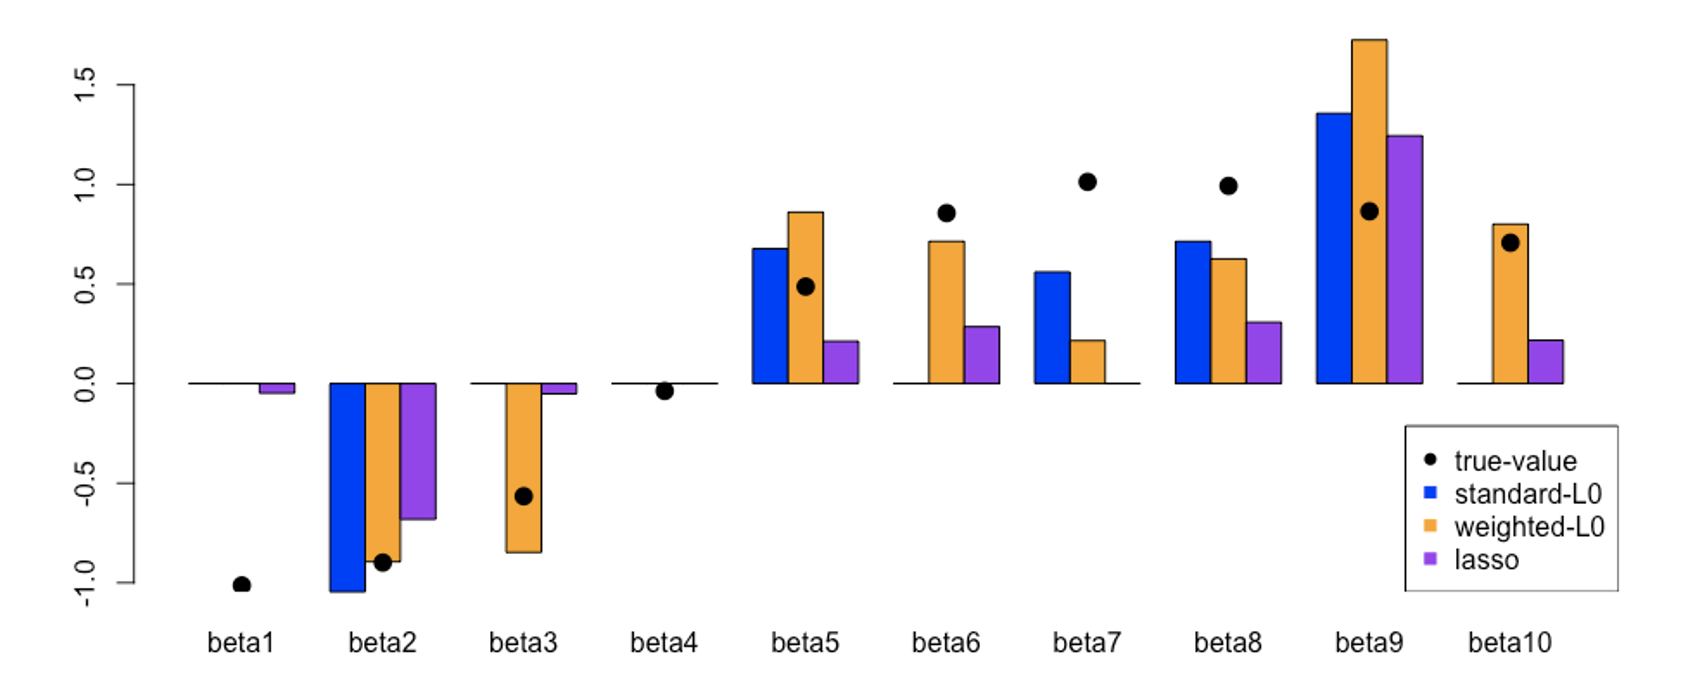
\includegraphics[width=\textwidth]{L_0}
  \caption{Comparison of signal estimates}
  \label{fig:L_0}
\end{figure}

The simulation results showed some potential for the weighted $L_0$ algorithm to improve feature selection in terms of accuracy and bias of the estimates. However, when we tried the proposed approximate solution to weighted projection in simulation, the results didn't show improvement in feature selection, and we haven't come up with a better solution to the weighted projection problem. 
